Wyst�puj� wyra�ne przegulowania, czas regulacji pozostawia sporo do �yczeni, a~sygna� steruj�cy, szczeg�lnie w~ przypadku DMC, ma tendencj� do nag�ej zmiany warto�ci.

\begin{figure}[H]
    \makebox[0.21\textwidth]{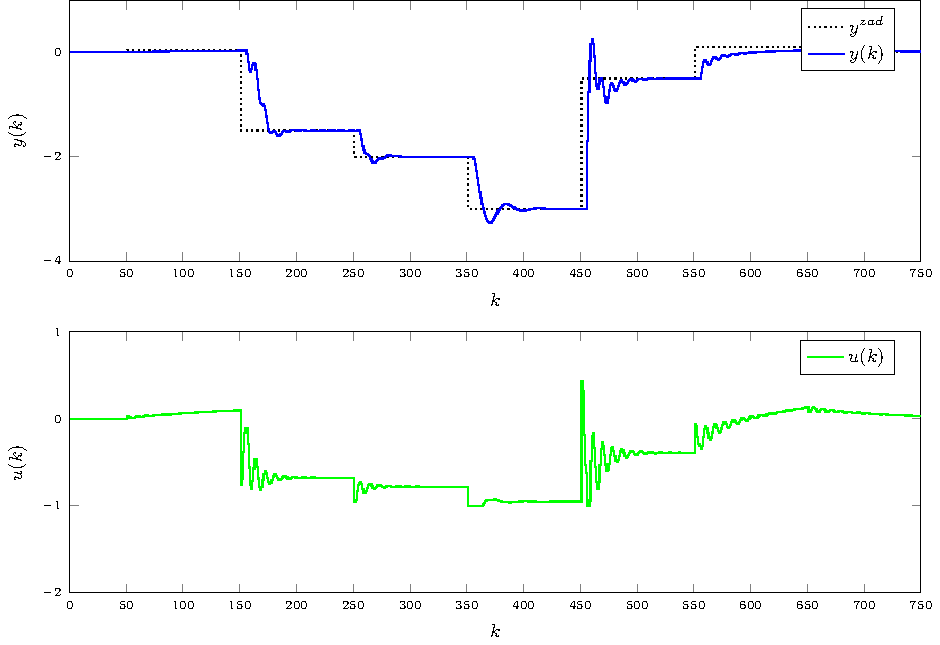
\includegraphics[width=0.2\paperwidth, height=0.15\paperheight]{data/Desired_plot_DMC_number_of_fuzzy_reg_1.pdf}}
\end{figure}

Warto zauwa�y�, �e przedstawiona trajektoria zadana jest dosy� specyficzna. Ukazuje ona tylko jedn� zmian� warto�ci zadanej o~znacznej amplitudzie, co nie pozwala dostrzec zachowania regulator�w przy jej znacznej w~przeciwnym kierunku. Najprawdopodobniej przy szerszym spektrum zmian regulatory ukaza�yby swoj� niedoskona�o�� w~znacznie wi�kszym stopniu.

